\section{Results}\label{sec:results}
% Budget: 4 pages. Every number below comes from results/tables/ (rerun src/pipeline.py to refresh).

\subsection{Full-sample networks}
Table~\ref{tab:static} (appendix) reports static connectedness estimated on the whole sample. The two dense estimators give almost the same total connectedness (Diebold--Yilmaz 81.9\%, lasso VAR 82.1\%), NETS gives 73.5\%, and the idiosyncratic component identified by FNETS gives only 34.2\%. The heatmap of Figure~\ref{fig:heatmap}(a) shows that Diebold--Yilmaz connectedness is spread widely across all pairs, with only mild regional clustering: the strongest pairs are Korea--Taiwan and the Indonesia--Malaysia--Philippines--Thailand block, and South Africa is a common source of shocks for almost every market. Once the common factor is removed (Figure~\ref{fig:heatmap}(b)), the remaining pairwise shares are concentrated in a few pairs (Korea--Taiwan above all), and the full-sample idiosyncratic partial-correlation network is empty (Figure~\ref{fig:network}, right panel). NETS retains 92 long-run partial-correlation links (60\% of all possible pairs). The lagged (Granger) dependence is very weak in all sparse estimators: lasso, NETS and FNETS keep only 2.5\%, 1.7\% and 0.3\% of the possible directed lag links in the rolling windows, so connectedness at the weekly frequency is overwhelmingly contemporaneous.

\subsection{Connectedness over time}
Figure~\ref{fig:total} shows the rolling total connectedness of each method. Diebold--Yilmaz connectedness moves between about 72\% and 89\%; the lasso VAR tracks it almost exactly (correlation 0.98). Because each estimate is dated at the end of its 104-week window, an episode affects the series for two years after it occurs. Connectedness is high at the start of the sample (88\%), falls to about 76\% in 2014--2015, rises to about 87\% in 2016--2017, is around 80\% in 2018--2019, and reaches its maximum (about 89\%) for windows that contain the March 2020 crash, falling back to the mid-70s after those weeks leave the window (2022--2023). NETS follows the same low-frequency pattern at a lower level (about 45--83\%) but is much noisier from one window to the next. FNETS idiosyncratic connectedness is flatter (mostly 43--55\%) and does not reproduce the 2020 peak. Figure~\ref{fig:overlay} shows why: the share of variance that FNETS attributes to the common component, which is between 47\% and 75\%, rises and falls with total connectedness, with a correlation of 0.95.

\subsection{Net transmitters and receivers}
Figure~\ref{fig:net} reports average net connectedness by country. In the Diebold--Yilmaz and lasso systems the main net transmitters are South Africa (+22 percentage points), South Korea (+16) and Taiwan (+12), and the main net receivers are Turkey ($-22$), Vietnam ($-21$) and Argentina ($-10$). NETS gives the same ranking at about half the magnitude (South Africa $+10$, Korea $+9$, Taiwan $+8$; Vietnam $-11$, Turkey $-11$, Argentina $-5$). The ranking of the countries' average net position is almost identical across DY, lasso and NETS (Spearman correlation between 0.96 and 0.99) but differs for FNETS (0.30 with DY). In the idiosyncratic network Taiwan (+9) and Indonesia (+8) are the main transmitters, Turkey is still the main receiver ($-6$), and Argentina is close to neutral ($+1.6$). Argentina is thus a receiver of the common component of emerging-market returns rather than of idiosyncratic shocks; in this sense it is one case among the 17 markets rather than an outlier.

\subsection{Comparison of methods}
Table~\ref{tab:criteria} summarizes the three criteria.

\paragraph{Density.} The Diebold--Yilmaz VAR is dense by construction. The sparse estimators remove almost all lagged links, and NETS and FNETS also sparsify the contemporaneous structure: the share of non-zero long-run partial correlations is 100\% for DY and lasso (which are implied by a full innovation covariance), 52\% for NETS and 7\% for FNETS. Among the generalized variance shares themselves, 35\% (DY) and 34\% (lasso) exceed the equal-share benchmark $1/N$, against 16\% for both NETS and FNETS.

\paragraph{Agreement.} Total connectedness is highly correlated between DY and the lasso VAR (0.98) and between DY and NETS (0.89), but not at all between DY and FNETS ($0.00$); the correlations of FNETS with lasso and NETS are $0.04$ and $0.08$. The same pattern holds for the matrices: the per-window Spearman correlation of the variance-decomposition entries with DY is 0.93 for lasso, 0.80 for NETS and $-0.06$ for FNETS, and the overlap of the strongest 10\% of links (Jaccard) is 0.61, 0.51 and 0.16. Agreement is lower for the networks that are sparse by design: for long-run partial correlations the Spearman correlation with DY is 0.33 (lasso) and 0.36 (NETS), while lasso and NETS agree more with each other (0.66). The Granger networks barely agree (Spearman at most 0.23), as expected given how few lag links survive.

\paragraph{Stability.} The standard deviation of total connectedness across windows is 5.1 (DY), 5.7 (lasso), 11.0 (NETS) and 4.6 (FNETS), but its mean absolute change from one window to the next is 0.7, 0.8, 4.6 and 3.0: the dense estimators move smoothly, while NETS and FNETS jump. The correlation between consecutive windows' variance-decomposition matrices is 0.97 (DY), 0.97 (lasso), 0.93 (NETS) and 0.82 (FNETS). For long-run partial-correlation links the overlap of the strongest 10\% between consecutive windows is 0.61, 0.64, 0.72 and 0.12, so NETS has the most persistent sparse structure and the FNETS idiosyncratic network is the least stable. The sharp one-window drops of the FNETS series coincide with windows in which the penalized idiosyncratic VAR retains several coefficients (correlation of $-0.72$ between total connectedness and the number of non-zero coefficients); we therefore read them as estimation noise in short windows and not as events.

\subsection{Common factor versus idiosyncratic connectedness}
FNETS selects one common factor in every window, which explains on average 58\% of the variance of the series. Total connectedness of the idiosyncratic VAR is 41\% lower than that of the DY VAR on average (median 42\%; between 26\% and 61\% across windows). The loss is stable across specifications (Table~\ref{tab:robustness}): 38\% with 78-week windows, 43\% with 130-week windows, 42\% without SPY and 41\% when windows that touch 2020 are removed, and it does not depend on the horizon. In the subsamples (Table~\ref{tab:static}), DY connectedness is 83.0\% in 2011--2019 and 73.5\% in 2021--2026, NETS falls from 69.6\% to 56.0\%, while idiosyncratic FNETS connectedness rises slightly (34.1\% to 39.6\%) as the common-factor variance share falls from 58\% to 47\%. A large part of the variation of DY connectedness over time is therefore variation in the weight of the common factor.

\begin{figure}[!t]
\centering
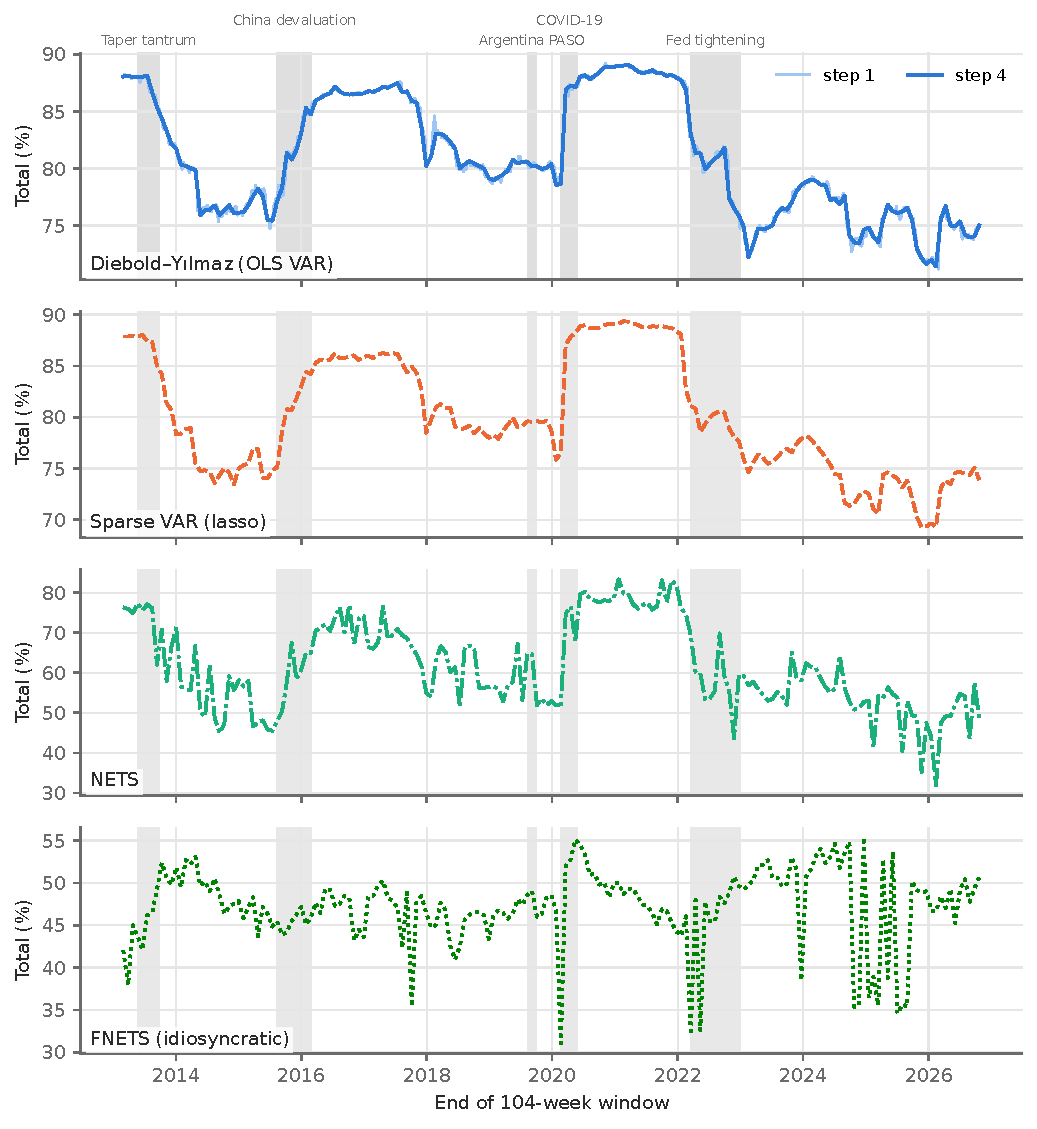
\includegraphics[width=\linewidth]{total_connectedness}
\caption{Total connectedness over time by method (104-week rolling windows, $H=4$, step 4). Estimates are dated at the end of the window. Shaded areas mark events.}
\label{fig:total}
\end{figure}

\begin{figure}[!t]
\centering
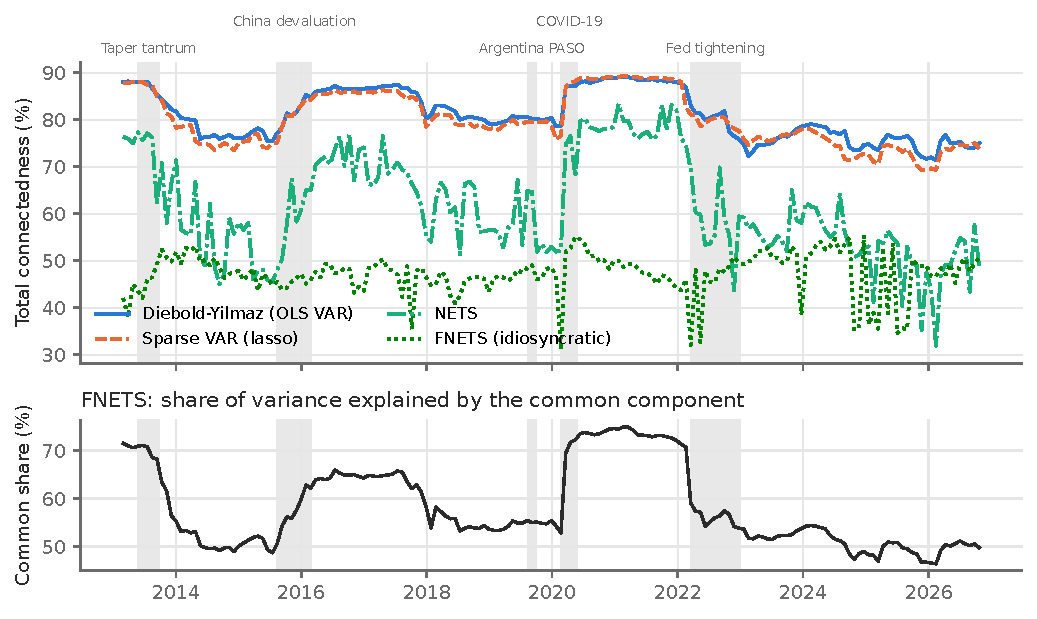
\includegraphics[width=\linewidth]{total_connectedness_overlay}
\caption{Top: total connectedness of all methods on a common scale. Bottom: FNETS share of variance explained by the common component.}
\label{fig:overlay}
\end{figure}

\begin{figure}[!t]
\centering
\begin{subfigure}{0.49\linewidth}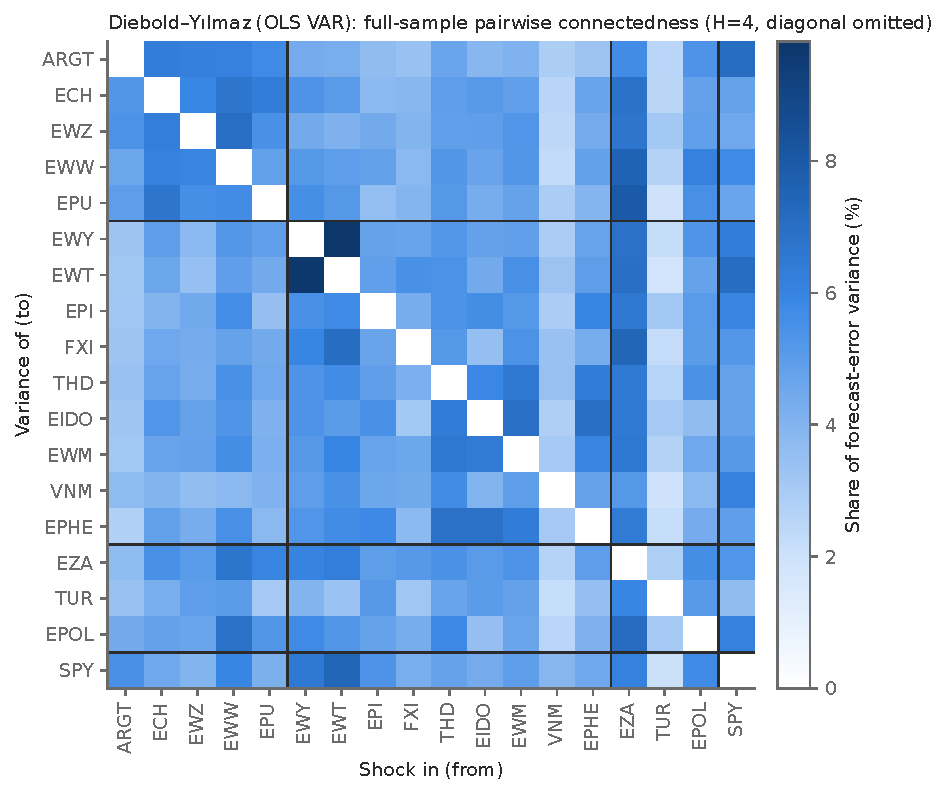
\includegraphics[width=\linewidth]{heatmap_dy}\caption{DY}\end{subfigure}
\begin{subfigure}{0.49\linewidth}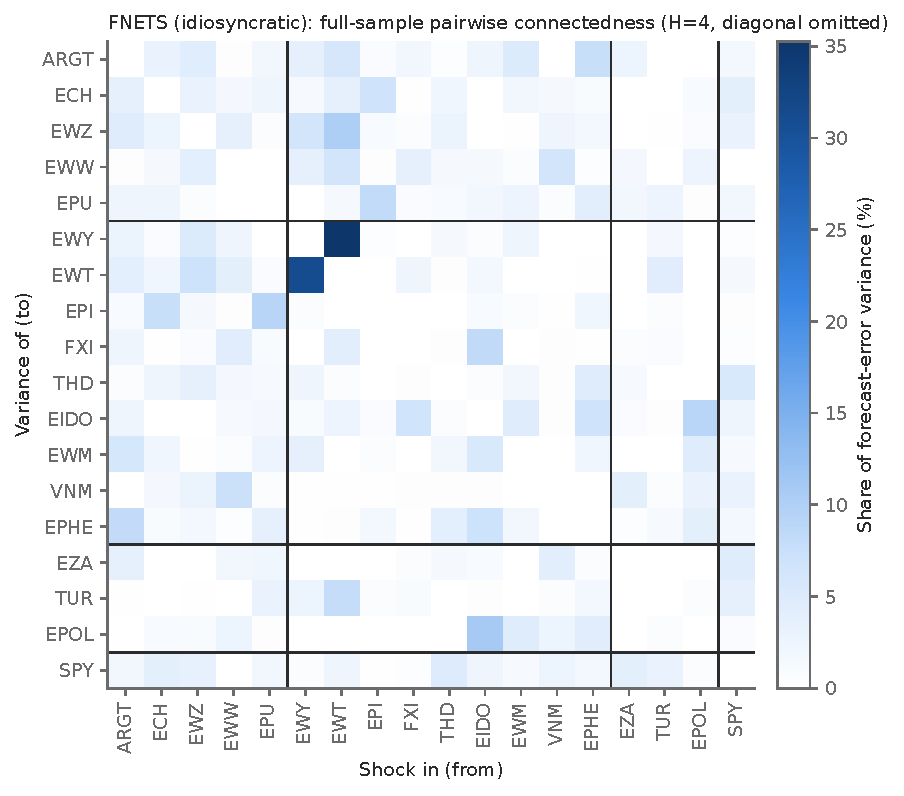
\includegraphics[width=\linewidth]{heatmap_fnets}\caption{FNETS (idiosyncratic)}\end{subfigure}
\caption{Full-sample pairwise connectedness, countries grouped by region (Latin America, Asia, EMEA, global).}
\label{fig:heatmap}
\end{figure}

\begin{figure}[!t]
\centering
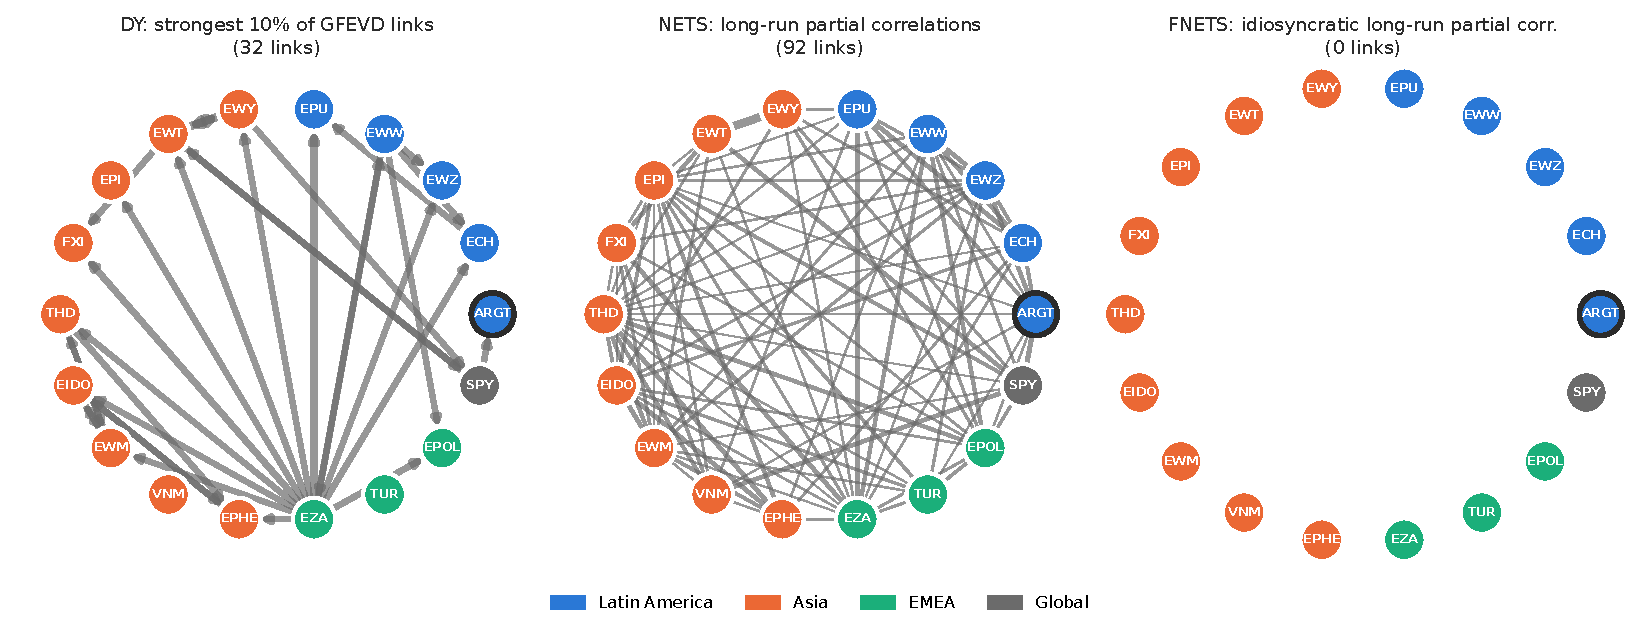
\includegraphics[width=\linewidth]{network_full_sample}
\caption{Full-sample networks. Node colors denote regions; ARGT is outlined. Left: strongest 10\% of Diebold--Yilmaz links. Center: NETS long-run partial correlations. Right: FNETS idiosyncratic long-run partial correlations (no links in the full sample).}
\label{fig:network}
\end{figure}

\begin{figure}[!t]
\centering
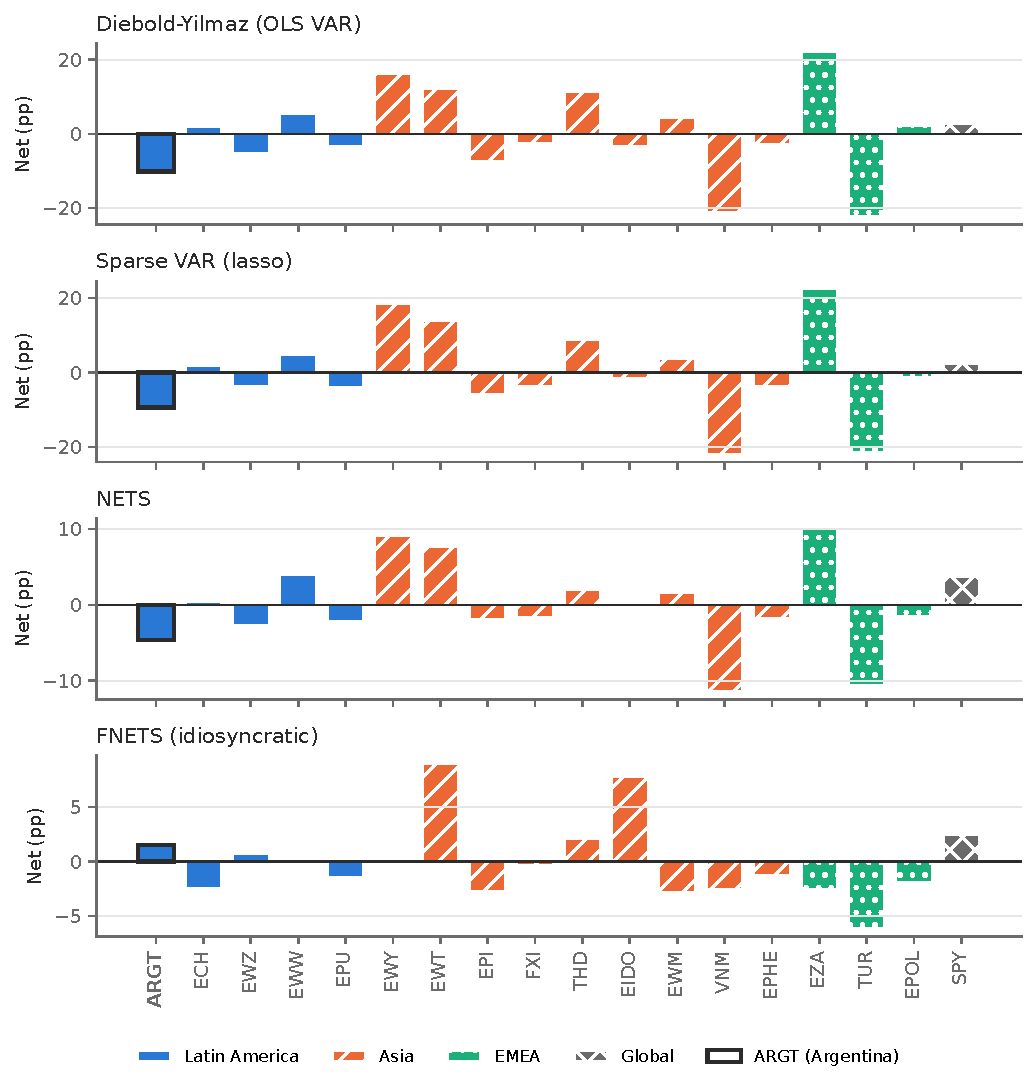
\includegraphics[width=\linewidth]{net_connectedness_by_country}
\caption{Average net connectedness by country (transmitters $>0$, receivers $<0$), in percentage points. ARGT outlined.}
\label{fig:net}
\end{figure}

\begin{table}[!t]
\centering\scriptsize
\caption{Comparison criteria across methods (179 windows, $w=104$, $H=4$). Densities in \%; agreement measured against DY; stability is the mean Spearman correlation (variance decomposition) and top-10\% Jaccard similarity (long-run partial correlations) between consecutive windows.}
\label{tab:criteria}
\resizebox{\linewidth}{!}{\input{\tablepath/comparison_criteria.tex}}
\end{table}
